\documentclass[conference]{IEEEtran}
\IEEEoverridecommandlockouts
% The preceding line is only needed to identify funding in the first footnote. If that is unneeded, please comment it out.
\usepackage[utf8]{inputenc} % allow utf-8 input
\usepackage[T1]{fontenc}    % use 8-bit T1 fonts
\usepackage{hyperref}       % hyperlinks
\usepackage{url}            % simple URL typesetting
\usepackage{booktabs}       % professional-quality tables
\usepackage{nicefrac}       % compact symbols for 1/2, etc.
\usepackage{microtype}      % microtypography
\usepackage{multicol}
\usepackage{multirow}
\usepackage{diagbox}
\usepackage{subfigure}
\usepackage{tabularx}
\usepackage{cite}
\usepackage{amsmath,amssymb,amsfonts}
\usepackage{algorithmic}
\usepackage{graphicx}
\usepackage{textcomp}
\usepackage{xcolor}
\usepackage{indentfirst}
\def\BibTeX{{\rm B\kern-.05em{\sc i\kern-.025em b}\kern-.08em
    T\kern-.1667em\lower.7ex\hbox{E}\kern-.125emX}}
\begin{document}
\bibliographystyle{IEEEtran}

\title{Principles of Data Science Project 4\\
Domain Adaptation}

\author{\IEEEauthorblockN{Hongzhou Liu}
\IEEEauthorblockA{517030910214}
\texttt{deanlhz@sjtu.edu.cn}
\and
\IEEEauthorblockN{Xuanrui Hong}
\IEEEauthorblockA{517030910227}
\texttt{hongxuanrui.1999@sjtu.edu.cn}
\and
\IEEEauthorblockN{Qilin Chen}
\IEEEauthorblockA{517030910155}
\texttt{1017856853@sjtu.edu.cn}
}

\maketitle

\begin{abstract}
In this project, we tried different domain adaptation methods on the Office-Home dataset, which contains 65 categories of things from 4 domains.
The four domains are Art, Clipart, Product and Real-World. In our experiments, we take Art, Clipart and Product as source domains and Real-World as target domain.
For traditional methods, we tried KMM, CORAL, GFK, TCA, and EasyTL. For deep learning methods, we only tried DAN due to the scarce of computation resources and time limitation.
We compared performances among those methods and discussed the difference among them. 
\end{abstract}

\begin{IEEEkeywords}
Domain Adaptation, Transfer Learning
\end{IEEEkeywords}

\section{Introduction}

In this project, we tried different unsupervised domain adaptation methods on the Office-Home dataset, which contains 65 categories of things from 4 domains. The four domains are Art, Clipart, Product and Real-World. There are two parts in this section. Firstly, we will introduce several traditional transfer learning
methods we used in our project, including KMM, CORAL, GFK TCA and EasyTL. Then we will introduce deep transfer learning method DAN to compare with the traditional transfer learning methods.

\subsection{Transfer Component Analysis (TCA)}


For domain adaptation, Transfer Component Analysis (TCA) \cite{Sinno2011Domain} tries to learn some transfer components across domains in a Reproducing Kernel Hilbert Space (RKHS) using Maximum Mean Discrepancy (MMD). It minimizes the distance between domain distributions by projecting data onto the learned transfer components.

The basic assumption of TCA is 
$$P\left(X_{s}\right) \neq P\left(X_{t}\right)$$
where $X_{s}$ denotes source domain data and $P\left(X_{s}\right)$ denotes its marginal distributions, $X_{t}$ denotes target domain data and $P\left(X_{t}\right)$ denotes its marginal distributions. The motivation of TCA is to find a map $\Phi$ which could preserve the most data properties after projection, which means obtain the most variance, i.e.
$$P\left(\phi\left(\mathbf{x}_{s}\right)\right) \approx P\left(\phi\left(\mathbf{x}_{t}\right)\right)$$
or we can find conditional distribution of the two will also be similar as:
$$
\left.\left.P\left(y_{s} \mid \phi\left(\mathbf{x}_{s}\right)\right)\right) \approx P\left(y_{t} \mid \phi\left(\mathbf{x}_{t}\right)\right)\right)
$$
We ccan give the maximum mean discrepancy (MMD) formula as:
$$
M M D(X, Y)=\left\|\frac{1}{n_{1}} \sum_{i=1}^{n_{1}} \Phi\left(x_{i}\right)-\frac{1}{n_{2}} \sum_{j=1}^{n_{2}} \Phi\left(y_{j}\right)\right\|^{2}
$$
where $n_1$, $n_2$ are the number of instances of the two domains. Then by changing the solution of this function to the solution of the kernel function, we can get: 
$$
\operatorname{Dist}\left(X_{S}^{\prime}, X_{T}^{\prime}\right)=\operatorname{tr}(K L)
$$
where
$$
K=\left[\begin{array}{ll}
K_{S, S} & K_{S, T} \\
K_{T, S} & K_{T, T}
\end{array}\right] \in \mathbb{R}^{\left(n_{1}+n_{2}\right) \times\left(n_{1}+n_{2}\right)}
$$,
then, Q Yang\cite{Sinno2011Domain} decomposed $K$ to transfer this problem to:
$$
\left\{\begin{array}{l}
\min t r\left(W^{T} K L K W\right)+\mu t r\left(W^{T} W\right) \\
\text { s.t. } W^{T} K H K W=I_{m}
\end{array}\right.
$$
Finally, we can get the solution $W*$ as the $m$ leading eigenvectors of
$$
(K L K+\mu I)^{-1} K H K
$$

\subsection{Easy Transfer Learning (EasyTL)}

Most traditional and deep learning migration algorithms are parametric methods, which require a lot of time and money to train those hyperparameters. In order to overcome these drawbacks, Easy Transfer Learning (EasyTL) \cite{Wang2019Easy} learns non-parametric transfer features through intra-domain alignment, and learns transmission classification through intra-domain programming. EasyTL can also improve the performance of existing TL methods through in-domain programming as the final classifier, the procedure of EasyTL can be shown in Fig. \ref{kFig1}. 

\begin{center}
	\begin{figure}[htbp]
		\centering
		\label{kFig1}
		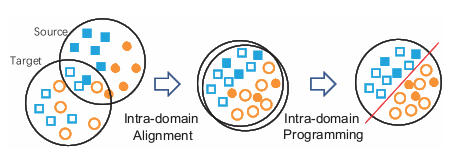
\includegraphics[width=8cm]{image/easyTL.png}
		\caption{procedure of EasyTL\cite{Wang2019Easy}}
	\end{figure}
\end{center}


\subsection{Deep Adaptation Network (DAN)}

Recent research shows that deep neural networks can learn transferable features, which can be well extended to new fields to adapt to tasks. Deep Adaptation Network (DAN) use deep net to optimize the loss function and distribution distance in Regenerative Nuclear Hilbert Space (RKHS) \cite{Long2015Learning}.

Denote $\mathcal{H}_{k}$ as the reproducing kernel Hilbert space (RKHS) endowed with a characteristic kernel $k$. The average embedding of the distribution $p$ in $\mathcal{H}_{k}$ is a unique element $k(p)$, making $\mathbf{E}_{\mathbf{x} \sim p} f(\mathbf{x})=\left\langle f( \mathbf{x}), \mu_{k}(p)\right\rangle_{\mathcal{H}_{k}}$ for all $f \in \mathcal{H}_{k}$. Define the MK-MMD $d_{k}(p, q)$between the probability distributions $p$ and $q$ as the average embedding distance RKHS of $p$ and $q$, and define the square formula of MK-MMD as

$$
d_{k}^{2}(p, q) \triangleq\left\|\mathbf{E}_{p}\left[\phi\left(\mathbf{x}^{s}\right)\right]-\mathbf{E}_{q}\left[\phi\left(\mathbf{x}^{t}\right)\right]\right\|_{\mathcal{H}_{k}}^{2}
$$
and the kernel defined by the multiple cores is
$$
\mathcal{K} \triangleq\left\{k=\sum_{u=1}^{m} \beta_{u} k_{u}: \sum_{u=1}^{m} \beta_{u}=1, \beta_{u} \geqslant 0, \forall u\right\}
$$

Global optimization goal consists of two parts: loss function and distribution distance. The loss function is used to measure the difference between the predicted value and the true value.

DAN use adaptive method based on mk-mmd and CNNs to onercome that the target domain has no or only limited label information, so it is impossible to adapt CNN directly to the target domain through fine-tuning, or it is easy to overfit. Fig. \ref{kFig2} gives a description of the proposed DAN model.

\begin{center}
	\begin{figure}[htbp]
		\centering
		\label{kFig2}
		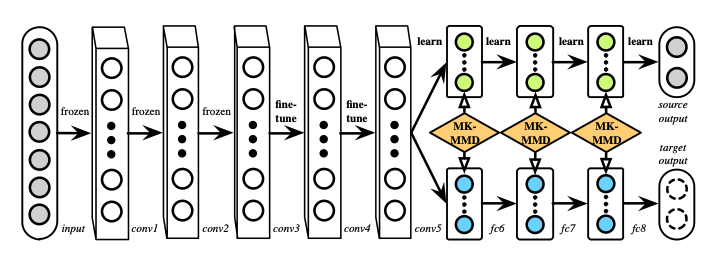
\includegraphics[width=8cm]{image/DAN.png}
		\caption{The DAN architecture for learning transferable features.Since deep features eventually transition from general to specific along the network, (1) the features extracted by convolutional layers conv1–conv3 are general, hence these layers are frozen, (2) the features extracted by layers conv4–conv5 are slightly less transferable, hence these layers are learned via fine-tuning, and (3) fully connected layers fc6–fc8 are tailored to fit specific tasks, hence they are not transferable and should be adapted with MK-MMD.\cite{Long2015Learning}}
	\end{figure}
\end{center}

DAN fine-tuned the source of the labeled examples, requiring that under the hidden representation of the fully connected layers $f$ $c6$ $f$ $c8$, the distribution of the source and target becomes similar. This can be achieved by adding a multi-layer adaptive regularizer (1) based on mk-mmd to the risk (3) of CNN:

$$
\min _{\Theta} \frac{1}{n_{a}} \sum_{i=1}^{n_{a}} J\left(\theta\left(\mathbf{x}_{i}^{a}\right), y_{i}^{a}\right)+\lambda \sum_{\ell=l_{1}}^{l_{2}} d_{k}^{2}\left(\mathcal{D}_{s}^{\ell}, \mathcal{D}_{t}^{\ell}\right)
$$


where $\lambda > 0$ is a penalty parameter, $l_1$ and $l_2$ are layer indices between which the regularizer is effective.

\section{Experiments}

In this part, we will show the experimental results and comparative analysis of the results through two types of traditional transfer learning methods and deep transfer learning methods.


\subsection{Transfer Component Analysis (TCA)}



\subsection{Easy Transfer Learning (EasyTL)}


\subsection{Deep Adaptation Network (DAN)}

\section{Conclusion}

\cite{lowe1999object}
\bibliography{Prj4}
\end{document}